\section{timer.h File Reference}
\label{timer_8h}\index{timer.h@{timer.h}}


This graph shows which files directly or indirectly include this file:\nopagebreak
\begin{figure}[H]
\begin{center}
\leavevmode
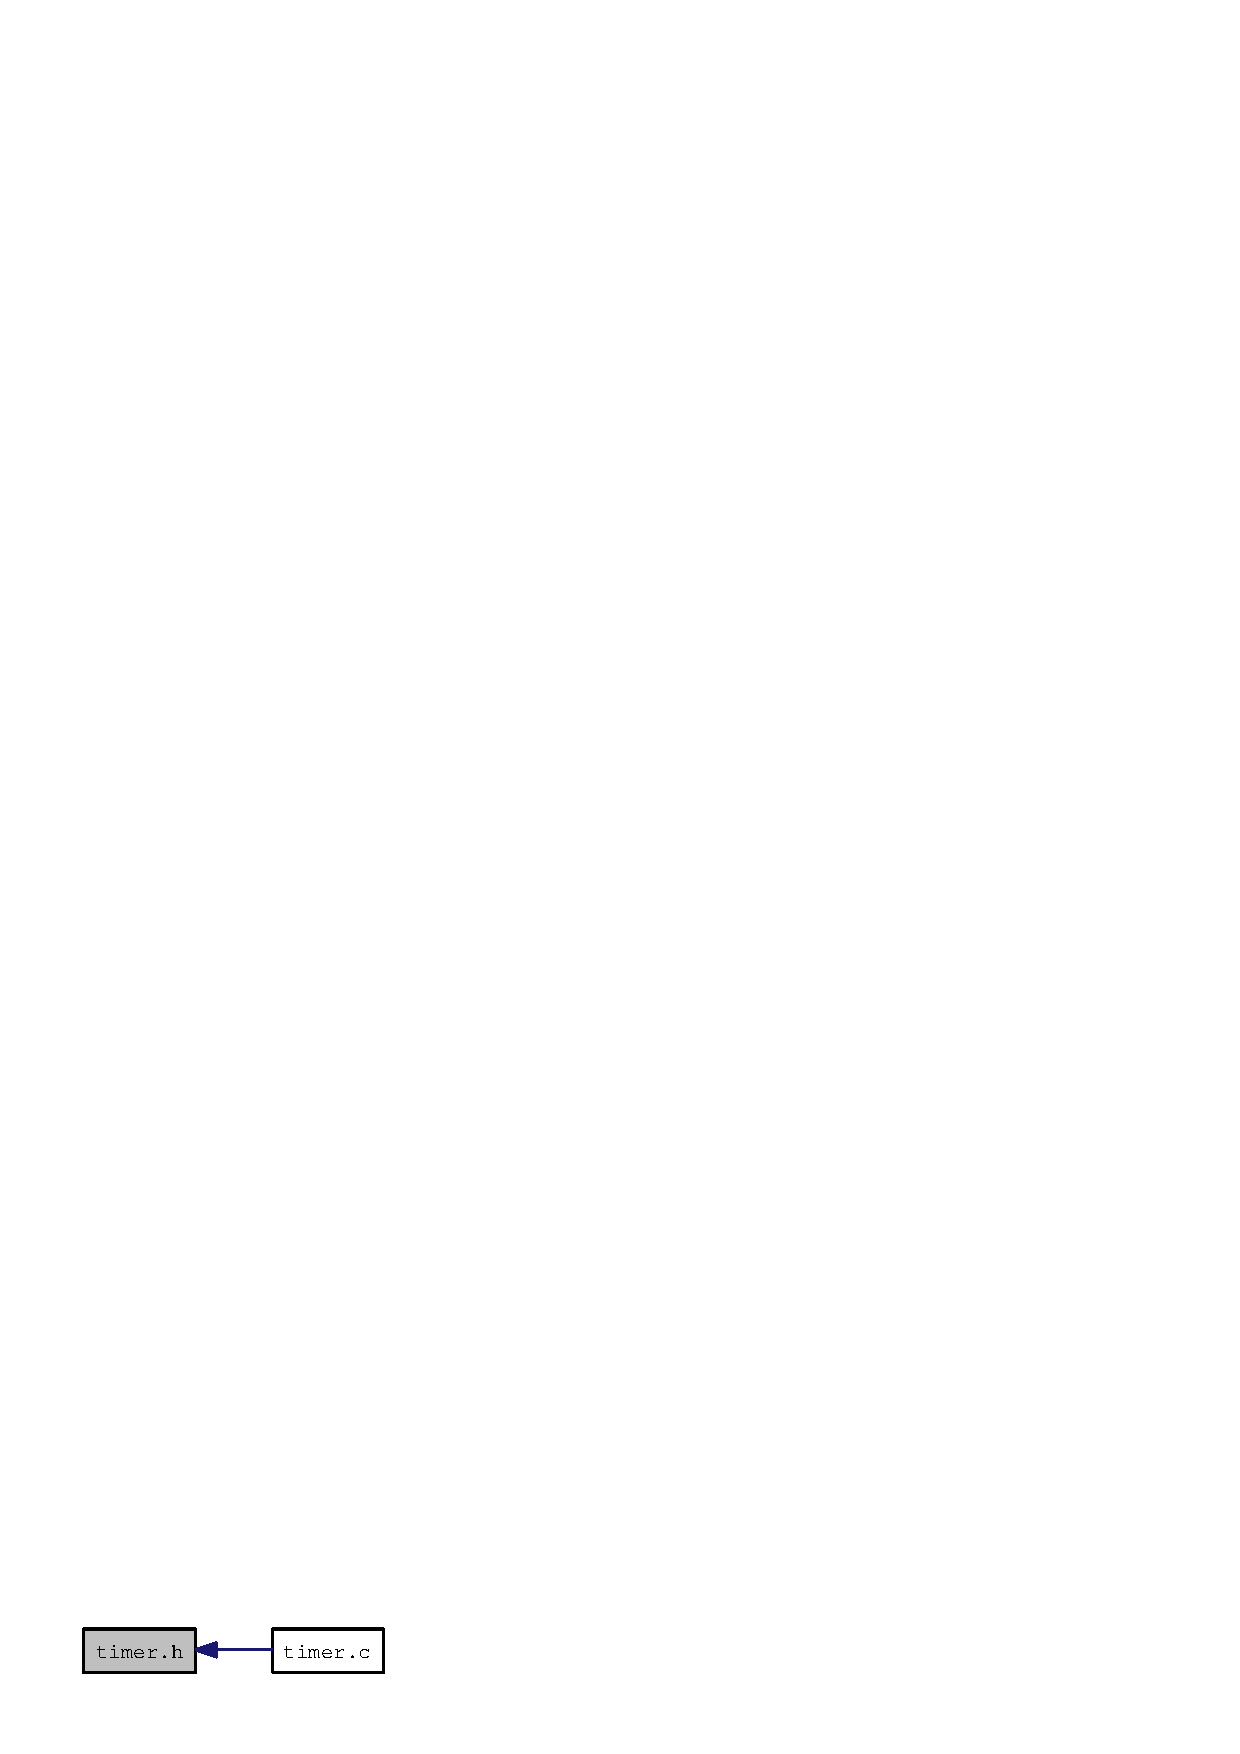
\includegraphics[width=94pt]{timer_8h__dep__incl}
\end{center}
\end{figure}
\subsection*{Defines}
\begin{CompactItemize}
\item 
\#define {\bf \_\-SFR\_\-ASM\_\-COMPAT}~1
\item 
\#define {\bf F\_\-CPU}~8000000
\item 
\#define {\bf TIMER\_\-INTERRUPT\_\-MODE}~1
\item 
\#define {\bf \_\-BV}(bit)~(1 $<$$<$ (bit))
\item 
\#define {\bf inb}(sfr)~\_\-SFR\_\-BYTE(sfr)
\item 
\#define {\bf inw}(sfr)~\_\-SFR\_\-WORD(sfr)
\item 
\#define {\bf outb}(sfr, val)~(\_\-SFR\_\-BYTE(sfr) = (val))
\item 
\#define {\bf outw}(sfr, val)~(\_\-SFR\_\-WORD(sfr) = (val))
\item 
\#define {\bf cbi}(sfr, bit)~(\_\-SFR\_\-BYTE(sfr) \&= $\sim$\_\-BV(bit))
\item 
\#define {\bf sbi}(sfr, bit)~(\_\-SFR\_\-BYTE(sfr) $|$= \_\-BV(bit))
\end{CompactItemize}
\subsection*{Functions}
\begin{CompactItemize}
\item 
void {\bf timer0Init} (uint8\_\-t mode, uint16\_\-t timerClockScale)
\begin{CompactList}\small\item\em Initialise Timer 0. \item\end{CompactList}\item 
uint16\_\-t {\bf timer0Read} (void)
\begin{CompactList}\small\item\em Read Timer 0. \item\end{CompactList}\end{CompactItemize}


\subsection{Define Documentation}
\index{timer.h@{timer.h}!_BV@{\_\-BV}}
\index{_BV@{\_\-BV}!timer.h@{timer.h}}
\subsubsection{\setlength{\rightskip}{0pt plus 5cm}\#define \_\-BV(bit)~(1 $<$$<$ (bit))}\label{timer_8h_11643f271076024c395a93800b3d9546}


Deal with MCUs with independent flag registers 

Definition at line 100 of file timer.h.\index{timer.h@{timer.h}!_SFR_ASM_COMPAT@{\_\-SFR\_\-ASM\_\-COMPAT}}
\index{_SFR_ASM_COMPAT@{\_\-SFR\_\-ASM\_\-COMPAT}!timer.h@{timer.h}}
\subsubsection{\setlength{\rightskip}{0pt plus 5cm}\#define \_\-SFR\_\-ASM\_\-COMPAT~1}\label{timer_8h_2a26f53e350366af6e573b70ef4036cd}


$<$ Special function register compatibility. 

Definition at line 35 of file timer.h.\index{timer.h@{timer.h}!cbi@{cbi}}
\index{cbi@{cbi}!timer.h@{timer.h}}
\subsubsection{\setlength{\rightskip}{0pt plus 5cm}\#define cbi(sfr, bit)~(\_\-SFR\_\-BYTE(sfr) \&= $\sim$\_\-BV(bit))}\label{timer_8h_e70baf5399951da1e7ad45a0ed890832}




Definition at line 105 of file timer.h.\index{timer.h@{timer.h}!F_CPU@{F\_\-CPU}}
\index{F_CPU@{F\_\-CPU}!timer.h@{timer.h}}
\subsubsection{\setlength{\rightskip}{0pt plus 5cm}\#define F\_\-CPU~8000000}\label{timer_8h_43bafb28b29491ec7f871319b5a3b2f8}




Definition at line 39 of file timer.h.\index{timer.h@{timer.h}!inb@{inb}}
\index{inb@{inb}!timer.h@{timer.h}}
\subsubsection{\setlength{\rightskip}{0pt plus 5cm}\#define inb(sfr)~\_\-SFR\_\-BYTE(sfr)}\label{timer_8h_5f2f31448ae0df9a545e0ca95e748f16}




Definition at line 101 of file timer.h.

Referenced by timer0Init(), and timer0Read().\index{timer.h@{timer.h}!inw@{inw}}
\index{inw@{inw}!timer.h@{timer.h}}
\subsubsection{\setlength{\rightskip}{0pt plus 5cm}\#define inw(sfr)~\_\-SFR\_\-WORD(sfr)}\label{timer_8h_b5e5eb4fcc7a892227a005faab343610}




Definition at line 102 of file timer.h.

Referenced by timer0Read().\index{timer.h@{timer.h}!outb@{outb}}
\index{outb@{outb}!timer.h@{timer.h}}
\subsubsection{\setlength{\rightskip}{0pt plus 5cm}\#define outb(sfr, val)~(\_\-SFR\_\-BYTE(sfr) = (val))}\label{timer_8h_b2639428f628a54f52f28ace148beb13}




Definition at line 103 of file timer.h.

Referenced by timer0Init().\index{timer.h@{timer.h}!outw@{outw}}
\index{outw@{outw}!timer.h@{timer.h}}
\subsubsection{\setlength{\rightskip}{0pt plus 5cm}\#define outw(sfr, val)~(\_\-SFR\_\-WORD(sfr) = (val))}\label{timer_8h_af663ae912dca7197d8ffab94ecbfb6d}




Definition at line 104 of file timer.h.

Referenced by timer0Init().\index{timer.h@{timer.h}!sbi@{sbi}}
\index{sbi@{sbi}!timer.h@{timer.h}}
\subsubsection{\setlength{\rightskip}{0pt plus 5cm}\#define sbi(sfr, bit)~(\_\-SFR\_\-BYTE(sfr) $|$= \_\-BV(bit))}\label{timer_8h_c4a5536d9bf092116f88b94797ddc882}




Definition at line 106 of file timer.h.

Referenced by timer0Init().\index{timer.h@{timer.h}!TIMER_INTERRUPT_MODE@{TIMER\_\-INTERRUPT\_\-MODE}}
\index{TIMER_INTERRUPT_MODE@{TIMER\_\-INTERRUPT\_\-MODE}!timer.h@{timer.h}}
\subsubsection{\setlength{\rightskip}{0pt plus 5cm}\#define TIMER\_\-INTERRUPT\_\-MODE~1}\label{timer_8h_2dd75713acf0fa9e97805a821b3a2dad}


Define this to allow code size to be reduced by removal of unwanted functions. Any or all may be used. 

Definition at line 45 of file timer.h.

\subsection{Function Documentation}
\index{timer.h@{timer.h}!timer0Init@{timer0Init}}
\index{timer0Init@{timer0Init}!timer.h@{timer.h}}
\subsubsection{\setlength{\rightskip}{0pt plus 5cm}void timer0Init (uint8\_\-t {\em mode}, uint16\_\-t {\em timerClock})}\label{timer_8h_b92fc98e45a0adae9832e4e037f79b41}


Initialise Timer 0. 

This function will initialise the timer with the mode of operation and the clock rate to be used. An error will be returned if the timer is busy.

Because ATMega64, ATMega128, ATMega103 offer different scale factors, there needs to be a conversion provided between the specification here and the scale setting. The additional clock settings provided for those MCUs are not used here, nor are the external clock settings of the remaining MCUs.

Timer 0 is typically an 8-bit timer and has very basic functionality. Some MCUs offer PWM capability while most do not.

\begin{Desc}
\item[Parameters:]
\begin{description}
\item[{\em mode}]Ignored for simple timers. \item[{\em timerClock}]00 Stopped 01 F\_\-CLK 02 F\_\-CLK/8 03 F\_\-CLK/64 04 F\_\-CLK/256 05 F\_\-CLK/1024\end{description}
\end{Desc}
The timer continues to run until it is stopped by calling this function with timerClock=0. At the moment, mode does nothing. 

Definition at line 80 of file timer.c.

References inb, outb, outw, and sbi.\index{timer.h@{timer.h}!timer0Read@{timer0Read}}
\index{timer0Read@{timer0Read}!timer.h@{timer.h}}
\subsubsection{\setlength{\rightskip}{0pt plus 5cm}uint16\_\-t timer0Read (void)}\label{timer_8h_7cf9215ace167364e5b1b2af46b0272d}


Read Timer 0. 

This function will return the current timer value as a 16 bit unsigned integer even if the timer is only 8 bit. This allows for a possibility of a 16 bit timer being at timer 0 (so far this is not the case in any MCU).

In the event of a 16 bit register, the hardware registers must be accessed high byte first. The avr-gcc compiler does this automatically.

\begin{Desc}
\item[Returns:]Timer Value. \end{Desc}


Definition at line 117 of file timer.c.

References inb, and inw.